\section{Methodology}
\ours follows the same framework as speculative decoding, where each decoding step primarily consists of three substeps: (1) generating candidates, (2) processing candidates, and (3) accepting candidates. For \ours, (1) is achieved by \ours heads, (2) is realized by tree attention, and since \ours heads are on top of the original model, the logits calculated in (2) can be used for substep (1) for the next decoding step. The final step (3) can be realized by either rejection sampling~\citep{leviathan2022fast,chen2023accelerating} or typical acceptance (Section~\ref{sec:typical_acceptance}). The overall pipeline is illustrated in Figure~\ref{fig:pipeline}.

In this section, we first introduce the key components of \ours, including \ours heads, and tree attention. Then, we present two levels of fine-tuning procedures for \ours to meet the needs of different use cases. Finally, we propose two extensions to \ours, including self-distillation and typical acceptance, to handle situations where no training data is available for \ours and to improve the efficiency of the decoding process, respectively.
\subsection{Key Components}
\subsubsection{\ours Heads}
\label{sec:medusa_heads}
In speculative decoding, subsequent tokens are predicted by an auxiliary draft model. This draft model must be small yet effective enough to generate continuations that the original model will accept. Fulfilling these requirements is a challenging task, and existing approaches~\citep{spector2023accelerating,miao2023specinfer} often resort to separately \emph{pre-training} a smaller model. This pre-training process demands substantial additional computational resources. For example, in \citep{miao2023specinfer}, a reported 275 NVIDIA A100 GPU hours were used. Additionally, separate pre-training can potentially create a distribution shift between the draft model and the original model, leading to continuations that the original model may not favor. \citet{chen2023accelerating} have also highlighted the complexities of serving multiple models in a distributed environment.

\textcolor{black}{To streamline and democratize the acceleration of LLM inference, we take inspiration from \citet{stern2018blockwise}, which utilizes parallel decoding for tasks such as machine translation and image super-resolution. \ours heads}
 are additional decoding heads appended to the last hidden states of the original model. Specifically, given the original model's last hidden states $h_t$ at position $t$, we add $K$ decoding heads to $h_t$. The $k$-th head is used to predict the token in the $(t+k+1)$-th position of the next tokens (the original language model head is used to predict the $(t+1)$-th position). The prediction of the $k$-th head is denoted as $p_t^{(k)}$, representing a distribution over the vocabulary, while the prediction of the original model is denoted as $p_t^{(0)}$. Following the approach of \citet{stern2018blockwise}, we utilize a single layer of feed-forward network with a residual connection for each head. We find that this simple design is sufficient to achieve satisfactory performance. The definition of the $k$-th head is outlined as:

\begin{align*}
p_t^{(k)} = \text{softmax}\left(W_2^{(k)} \cdot \left(\text{SiLU}(W_1^{(k)} \cdot h_t)+h_t\right)\right),\\
\text{where } W_2^{(k)}\in\mathbb{R}^{d\times V}, W_1^{(k)}\in\mathbb{R}^{d\times d}.
\end{align*}

\textcolor{black}{$d$ is the output dimension of the LLM's last hidden layer and $V$ is the vocabulary size.}
\textcolor{black}{We initialize $W_2^{(k)}$ identically to the original language model head, and $W_1^{(k)}$ to zero.}
This aligns the initial prediction of \ours heads with that of the original model. The SiLU activation function~\citep{elfwing2017sigmoidweighted} is employed following the Llama models~\citep{touvron2023llama}.

Unlike a draft model, \ours heads are trained in conjunction with the original backbone model, which can remain \emph{frozen} during training (\ours-1) or be trained together (\ours-2). This method allows for fine-tuning large models even on a single GPU, taking advantage of the powerful base model's learned representations. Furthermore, it ensures that the distribution of the \ours heads aligns with that of the original model, thereby mitigating the distribution shift problem. Additionally, since the new heads consist of just a single layer akin to the original language model head, \ours does not add complexity to the serving system design and is friendly to distributed settings. We will discuss the training recipe for \ours heads in Section~\ref{sec:training_recipe}.

\subsubsection{Tree Attention}
\label{sec:tree_attention}
Through \ours heads, we obtain probability predictions for the subsequent $K+1$ tokens. These predictions enable us to create length-$K+1$ continuations as candidates. While the speculative decoding studies~\citep{leviathan2022fast,chen2023accelerating} suggest sampling a single continuation as the candidate, leveraging multiple candidates during decoding can enhance the expected acceptance length within a decoding step. Nevertheless, more candidates can also raise computational demands. To strike a balance, we employ a tree-structured attention mechanism to process multiple candidates concurrently.
\begin{figure}[ht]
    \centering
    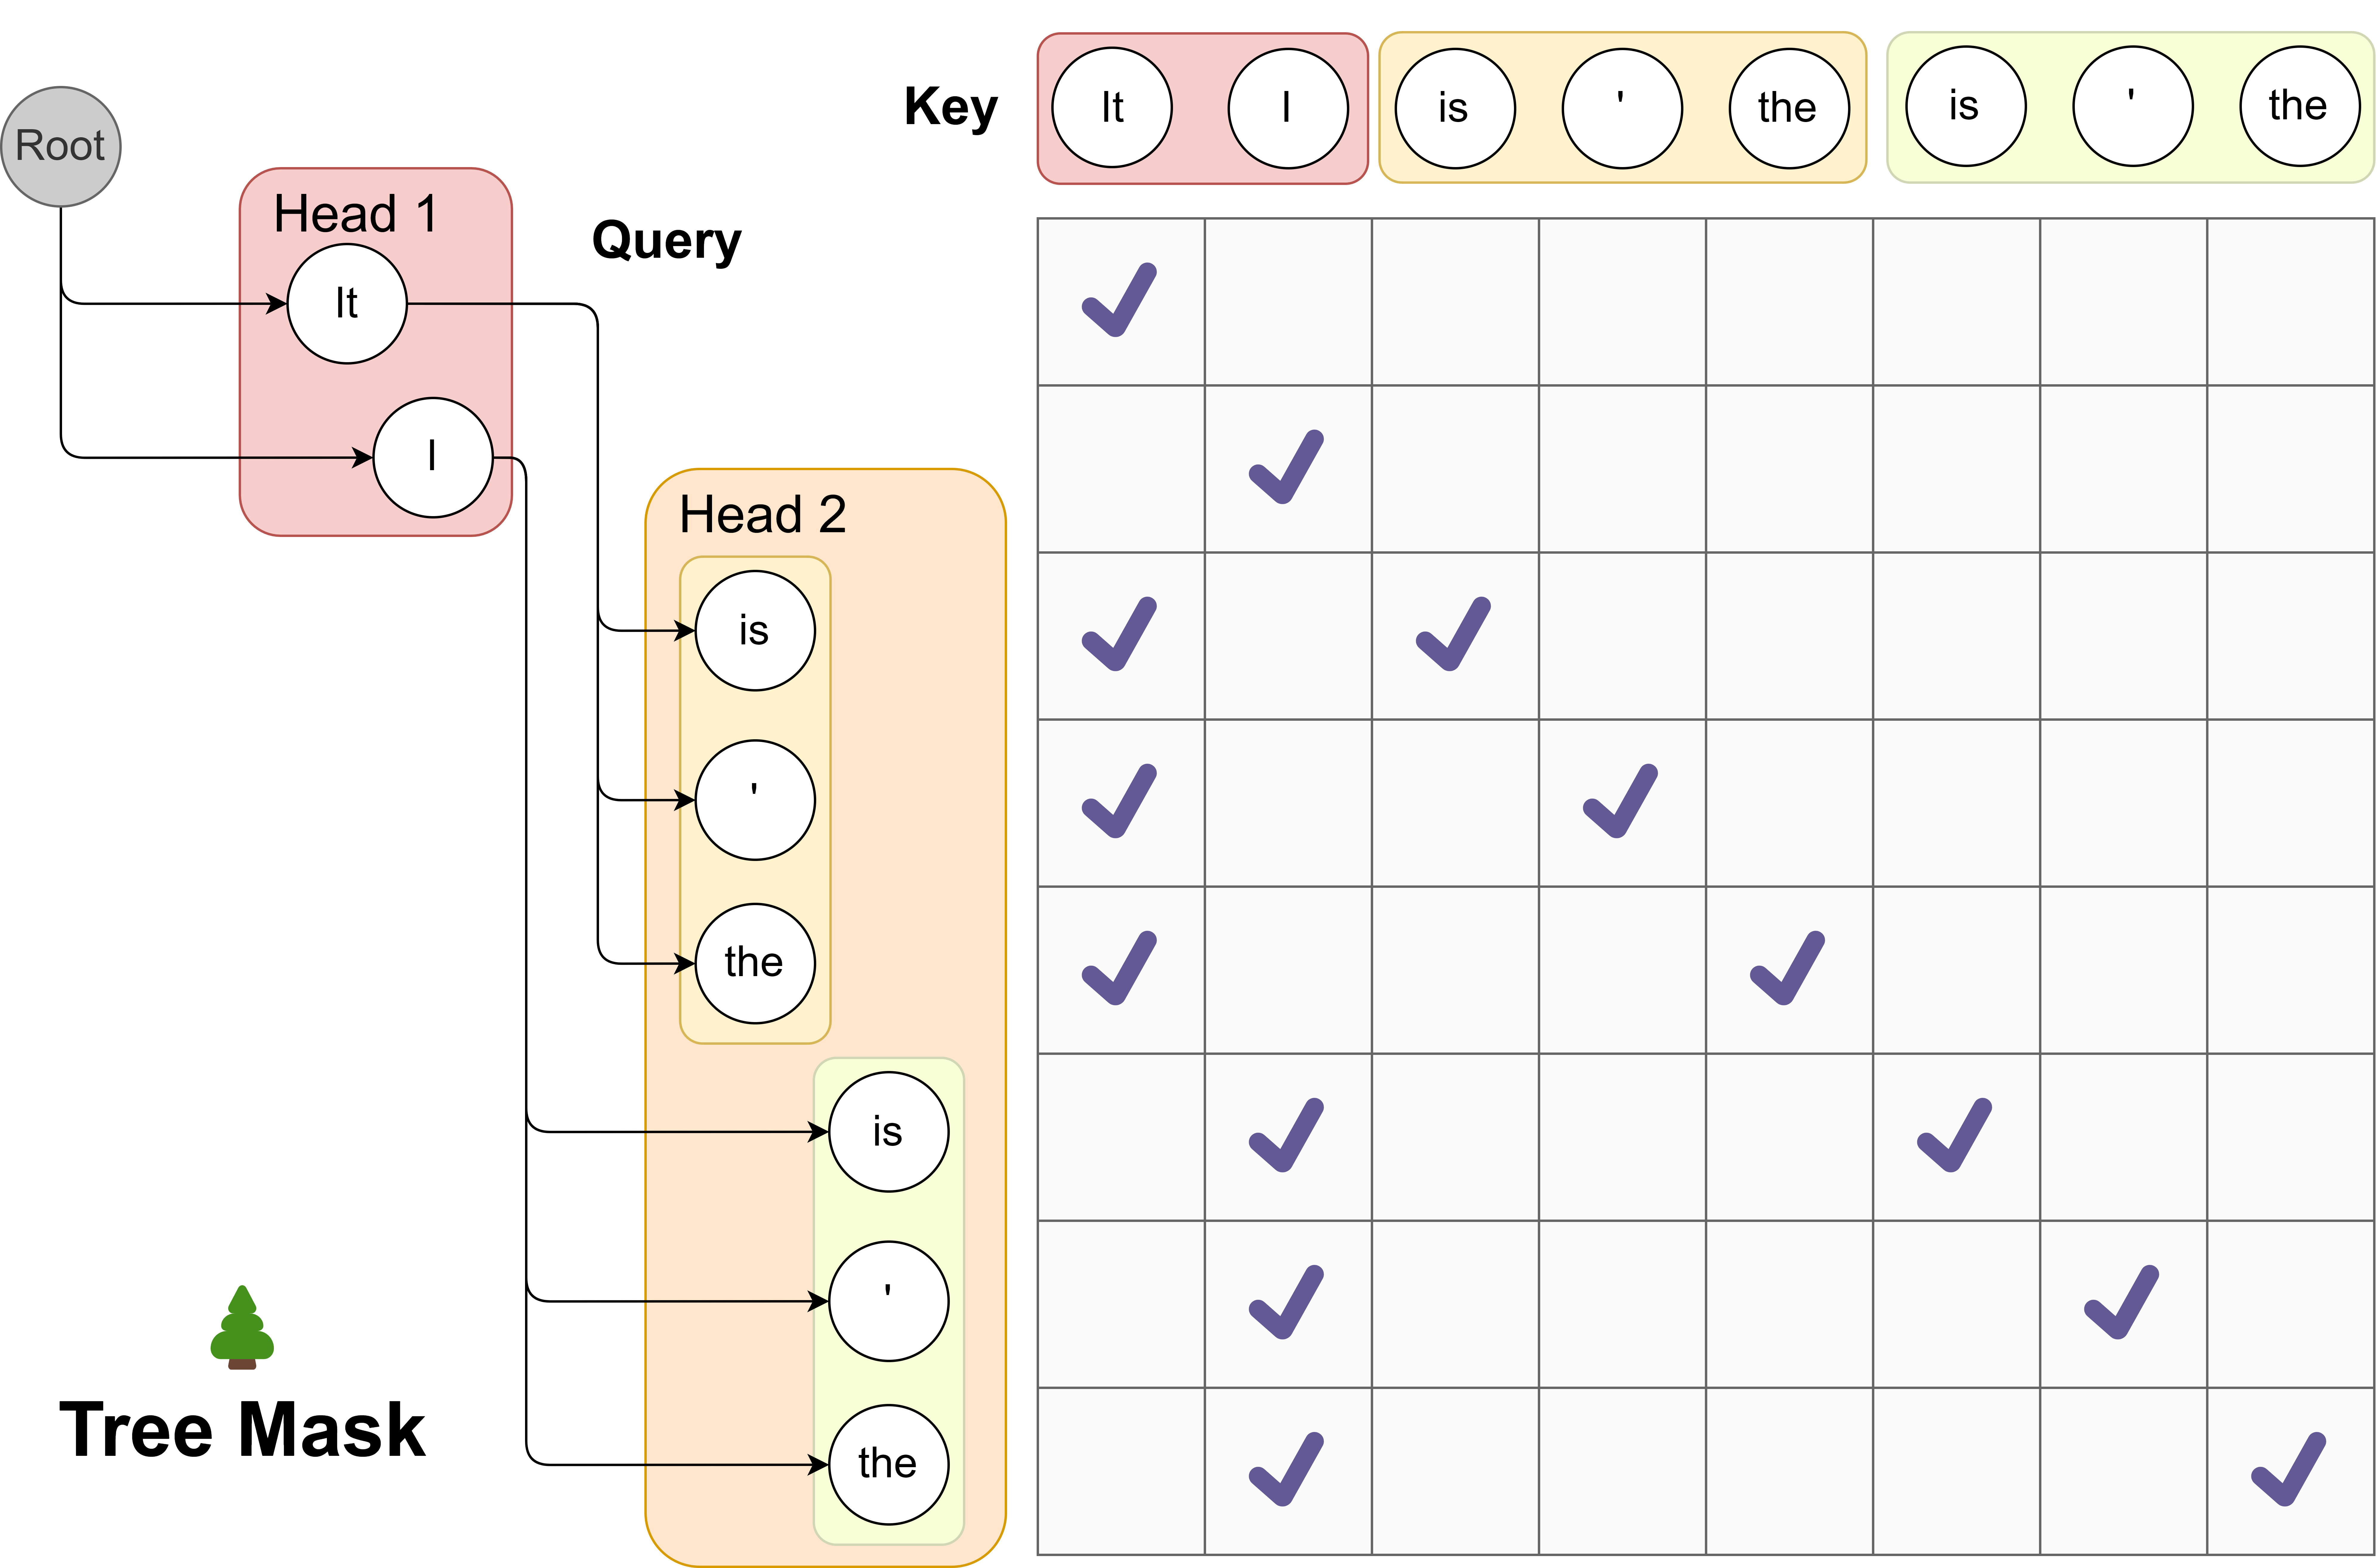
\includegraphics[width=0.45\textwidth]{tree_attention.png}
    \caption{
    We demonstrates the use of tree attention to process multiple candidates concurrently. As exemplified, the top-2 predictions from the first \ours head and the top-3 from the second result in a total of $2\times3=6$ candidates. Each of these candidates corresponds to a distinct branch within the tree structure. To guarantee that each token only accesses its predecessors, we devise an attention mask that exclusively permits attention flow from the current token back to its antecedent tokens. The positional indices for positional encoding are adjusted in line with this structure.}
    \label{fig:tree_attention}
\end{figure}
This attention mechanism diverges from the traditional causal attention paradigm. Within this framework, only tokens from the same continuation are regarded as historical data. Drawing inspiration from the concept of embedding graph structures into attention as proposed in the graph neural network domain~\citep{ying2021transformers}, we incorporate the tree structure into our attention mask, visualized in Figure~\ref{fig:tree_attention}. Remarkably, similar ideas have also been explored in independent works like \citet{miao2023specinfer,spector2023accelerating}, where they follow a bottom-up approach and construct the tree by merging multiple candidates generated by a draft model. In our method, we instead take a top-down approach to build the tree thanks to the structure of candidates generated by \ours heads. For a given $k$-th head, its top-$s_k$ predictions serve as the basis for candidate formation, where $s_k$ is a designated hyperparameter. These candidates are established by determining the Cartesian product of the top-$s_k$ predictions from each head. For instance, in Figure~\ref{fig:tree_attention}, with $s_1=2$ and $s_2=3$, each first head prediction can be succeeded by any prediction from the second head. This leads to a tree structure where $s_k$ branches exist at the $k$-th level (considering a virtual root as the $0$-level, in practice, this $0$-level is for the prediction of the language model head of the original model, which can be sampled independently). Within this tree, only a token's predecessors are seen as historical context, and our attention mask ensures that the attention is only applied on a token's predecessors. By employing this mask and properly setting the positional indices for positional encoding, we can process numerous candidates simultaneously without the need to expand the batch size. The cumulative number of new tokens is calculated as $\sum_{k=1}^K \prod_{i=1}^k s_i$.

In this section, we demonstrate the most simple and regular way to construct the tree structure by taking the Cartesian product. However, it is possible to construct the tree structure in a more sophisticated way and exploit the unbalanced accuracy of different top predictions of different heads. We will discuss this in Section~\ref{sec:optimized_tree_construction}.
\subsection{Training Strategies}
\label{sec:training_recipe}
At the most basic level, we can train \ours heads by freezing the backbone model and fine-tuning \ours heads. However, training the backbone in conjunction with the \ours heads can significantly enhance the accuracy of the \ours heads. Depending on the computational resources and the specific reqirements of the use case, we propose two levels of training strategies for \ours heads.

In this section, we assume the availability of a training dataset that aligns with the target model’s output distribution. This could be the dataset used for Supervised Fine-Tuning (SFT) of the target model. We will discuss eliminating the need for such a dataset using a self-distillation approach in Section~\ref{sec:self_distillation}.
\subsubsection{\ours-1: Frozen Backbone}
\label{sec:frozen_backbone}
To train \ours heads with a frozen backbone model, we can use the cross-entropy loss between the prediction of \ours heads and the ground truth. Specifically, given the ground truth token $y_{t+k+1}$ at position $t+k+1$, the loss for the $k$-th head is $\mathcal{L}_k = -\log p_t^{(k)}(y_{t+k+1})$ where $p_t^{(k)}(y)$ denotes the probability of token $y$ predicted by the $k$-th head. We also observe that $\mathcal{L}_k$ is larger when $k$ is larger, which is reasonable since the prediction of the $k$-th head is more uncertain when $k$ is larger. Therefore, we can add a weight $\lambda_k$ to $\mathcal{L}_k$ to balance the loss of different heads. And the total \ours loss is:
\begin{align}
    \label{eq:loss_medusa_1}
    \mathcal{L}_{\text{\ours-1}} = \sum_{k=1}^K -\lambda_k\log p_t^{(k)}(y_{t+k+1}).
\end{align}

In practice, we set $\lambda_k$ as the $k$-th power of a constant like $0.8$. Since we only use the backbone model for providing the hidden states, we can use a quantized version of the backbone model to reduce the memory consumption. This introduces a more democratized way to accelerate LLM inference, as with the quantization, \ours can be trained for a large model on a single consumer GPU similar to QLoRA~\citep{dettmers2023qlora}. The training only takes a few hours (e.g., 5 hours for \ours-1 on Vicuna 7B model with a single NVIDIA A100 PCIE GPU to train on 60k ShareGPT samples).
\subsubsection{\ours-2: Joint Training}
\label{sec:joint_training}
To further improve the accuracy of \ours heads, we can train \ours heads together with the backbone model. However, this requires a special training recipe to preserve the backbone model's next-token prediction capability and output quality. To achieve this, we propose three strategies:
\begin{itemize}
    \item \textbf{Combined loss}: To keep the backbone model's next-token prediction capability, we need to add the cross-entropy loss of the backbone model $\mathcal{L}_{\text{LM}}=-\log p_t^{(0)}(y_{t+1})$ to the \ours loss. We also add a weight $\lambda_0$ to balance the loss of the backbone model and the \ours heads. Therefore, the total loss is:
    \begin{align}
        \label{eq:loss_medusa_2}
        \mathcal{L}_{\text{\ours-2}} = \mathcal{L}_{\text{LM}} + \lambda_0\mathcal{L}_{\text{\ours-1}}.
    \end{align}
    \item \textbf{Differential learning rates}: Since the backbone model is already well-trained and the \ours heads need more training, we can use separate learning rates for them to enable faster convergence of \ours heads while preserving the backbone model's capability.
    \item \textbf{Heads warmup}: Noticing that at the beginning of training, the \ours heads have a large loss, which leads to a large gradient and may distort the backbone model's parameters. Following the idea from \citet{kumar2022finetuning}, we can employ a two-stage training process. In the first stage, we only train the \ours heads as \ours-1. In the second stage, we train the backbone model and \ours heads together with a warmup strategy. Specifically, we first train the backbone model for a few epochs, then train the \ours heads together with the backbone model. Besides this simple strategy, we can also use a more sophisticated warmup strategy by gradually increasing the weight $\lambda_0$ of the backbone model's loss. We find both strategies work well in practice.
\end{itemize}
Putting these strategies together, we can train \ours heads together with the backbone model without hurting the backbone model's capability. Moreover, this recipe can be applied together with Supervised Fine-Tuning (SFT), enabling us to get a model with native \ours support.
\subsubsection{How to Select the Number of Heads}
Empirically, we found that five heads are sufficient at most. Therefore, we recommend training with five heads and referring to the strategy described in Section~\ref{sec:optimized_tree_construction} to determine the optimal configuration of the tree attention. With optimized tree attention, sometimes three or four heads may be enough for inference. In this case, we can ignore the redundant heads without overhead.

\subsection{Extensions}
\subsubsection{Typical Acceptance}
\label{sec:typical_acceptance}
In speculative decoding papers~\citep{leviathan2022fast,chen2023accelerating}, authors employ rejection sampling to yield diverse outputs that align with the distribution of the original model. However, subsequent implementations~\citep{gante2023assisted,spector2023accelerating} reveal that this sampling strategy results in diminished efficiency as the sampling temperature increases. Intuitively, this can be comprehended in the extreme instance where the draft model is the same as the original one\textcolor{black}{:} 
Using greedy decoding, all output of the draft model will be accepted, therefore maximizing the efficiency. 
Conversely, rejection sampling introduces extra overhead, as the draft model and the original model are sampled independently. Even if their distributions align perfectly, the output of the draft model may still be rejected.

However, in real-world scenarios, sampling from language models is often employed to generate diverse responses, and the temperature parameter is used merely to modulate the ``creativity'' of the response. Therefore, higher temperatures should result in more opportunities for the original model to accept the draft model's output. We ascertain that it is typically unnecessary to match the distribution of the original model. Thus, we propose employing a \emph{typical acceptance} scheme to select plausible candidates rather than using rejection sampling. This approach draws inspiration from truncation sampling studies~\citep{hewitt2022truncation} (refer to \textcolor{black}{Appendix}~\ref{sec:related_work} for an in-depth explanation). Our objective is to choose candidates that are \emph{typical}, meaning they are not exceedingly improbable to be produced by the original model. We use the prediction probability from the \emph{original model} as a natural gauge for this and establish a threshold based on the prediction distribution to determine acceptance. Specifically, given $x_1, x_2, \cdots, x_n$ as context, when evaluating the candidate sequence \textcolor{black}{$(x_{n+1}, x_{n+2}, \cdots, x_{n+K+1})$ }(composed by top predictions of the original language model head and \ours heads), we consider the condition
\begin{align*}
p_{\text{original}}(x_{n+k}|x_1, x_2, \cdots, x_{n+k-1}) > \\\min\rbr{\epsilon, \delta\exp\rbr{-H(p_{\text{original}}(\cdot|x_1, x_2, \cdots, x_{n+k-1}))}},
\end{align*}
where $H(\cdot)$ denotes the entropy function, and $\epsilon, \delta$ are \textcolor{black}{the hard threshold and the entropy-dependent
threshold respectively}. This criterion is adapted from \citet{hewitt2022truncation} and rests on two observations: (1) tokens with relatively high probability are meaningful, and (2) when the distribution's entropy is high, various continuations may be deemed reasonable. During decoding, every candidate is evaluated using this criterion, and a \emph{prefix} of the candidate is accepted if it satisfies the condition. To guarantee the generation of at least one token at each step, we apply \emph{greedy decoding} for the first token and \emph{unconditionally} accept it while employing typical acceptance for subsequent tokens. The final prediction for the current step is determined by the \emph{longest accepted prefix} among all candidates.

Examining this scheme leads to several insights. Firstly, when the temperature is set to $0$, it reverts to greedy decoding, as only the most probable token possesses non-zero probability. As the temperature surpasses $0$, the outcome of greedy decoding will consistently be accepted with appropriate $\epsilon, \delta$, since those tokens have the maximum probability, yielding maximal speedup. Likewise, in general scenarios, an increased temperature will correspondingly result in longer accepted sequences, as corroborated by our experimental findings.

Empirically, we verify that typical acceptance can achieve a better speedup while maintaining a similar \textcolor{black}{generation quality} as shown in Figure~\ref{fig:threshold_ablation}.
\subsubsection{Self-Distillation}
\label{sec:self_distillation}
In Section~\ref{sec:training_recipe}, we assume the existence of a training dataset that matches the target model's output distribution. However, this is not always the case. For example, the model owners may only release the model without the training data, or the model may have gone through a Reinforcement Learning with Human Feedback (RLHF) procedure, which makes the output distribution of the model different from the training dataset. To tackle this issue, we propose an automated self-distillation pipeline to use the model itself to generate the training dataset for \ours heads, which matches the output distribution of the model.

The dataset generation process is straightforward. We first take a public seed dataset from a domain similar to the target model; for example, using the ShareGPT~\citep{sharegpt2023} dataset for chat models. Then, we simply take the prompts from the dataset and ask the model to reply to the prompts. In order to obtain multi-turn conversation samples, we can sequentially feed the prompts from the seed dataset to the model. Or, for models like Zephyr 7B~\citep{tunstall2023zephyr}, which are trained on both roles of the conversation, they have the ability to self-talk, and we can simply feed the first prompt and let the model generate multiple rounds of conversation.

For \ours-1, this dataset is sufficient for training \ours heads. However, for \ours-2, we observe that solely using this dataset for training the backbone and \ours heads usually leads to a lower generation quality. In fact, even without training \ours heads, training the backbone model with this dataset will lead to performance degradation. This suggests that we also need to use the original model's probability prediction instead of using the ground truth token as the label for the backbone model, similar to classic knowledge distillation works~\citep{kim2016sequencelevel}. Concretely, the loss for the backbone model is:
\begin{align*}
    \mathcal{L}_{\text{LM-distill}} = KL(p_{\text{original},t}^{(0)}||p_t^{(0)}),
\end{align*}
where $p_{\text{original},t}^{(0)}$ denotes the probability distribution of the original model's prediction at position $t$.

However, naively, to obtain the original model's probability prediction, we need to maintain two models during training, increasing the memory requirements. To further alleviate this issue, we propose a simple yet effective way to exploit the self-distillation setup. We can use a parameter-efficient adapter like LoRA~\citep{hu2021lora} for fine-tuning the backbone model. In this way, the original model is simply the model with the adapter turned off. Therefore, the distillation does not require additional memory consumption. Together, this self-distillation pipeline can be used to train \ours-2 without hurting the backbone model's capability and introduce almost no additional memory consumption. Lastly, one tip about using self-distillation is that it is preferable to use LoRA without quantization in this case, otherwise, the teacher model will be the quantized model, which may lead to a lower generation quality.

\subsubsection{Searching for the Optimized Tree Construction}
\label{sec:optimized_tree_construction}
In Section~\ref{sec:tree_attention}, we present the simplest way to construct the tree structure by taking the Cartesian product. However, with a fixed budget for the number of total nodes in the tree, a regular tree structure may not be the best choice. Intuitively, those candidates composed of the top predictions of different heads may have different accuracies. Therefore, we can leverage an estimation of the accuracy to construct the tree structure.

Specifically, we can use a calibration dataset and calculate the accuracies of the top predictions of different heads. Let $a_k^{(i)}$ denote the accuracy of the $i$-th top prediction of the $k$-th head\footnote{Here, the accuracy is defined for the single top $i$-th token, i.e., this accuracy is equal to top-$i$ accuracy minus top-$(i-1)$ accuracy.}. Assuming the accuracies are independent, we can estimate the accuracy of a candidate sequence composed by the top $\sbr{i_1, i_2, \cdots, i_k}$ predictions of different heads as $\prod_{j=1}^k a_j^{(i_j)}$. Let $I$ denote the set of all possible combinations of $\sbr{i_1, i_2, \cdots, i_k}$ and each element of $I$ can be mapped to a node of the tree (not only leaf nodes but all nodes are included). Then, the expectation of the acceptance length of a candidate sequence is:
\begin{align*}
    \sum_{\sbr{i_1, i_2, \cdots, i_k}\in I}\prod_{j=1}^k a_j^{(i_j)}.
\end{align*}
Thinking about building a tree by adding nodes one by one, the contribution of a new node to the expectation is exactly the accuracy associated with the node. Therefore, we can greedily add nodes to the tree by choosing the node that is connected to the current tree and has the highest accuracy. This process can be repeated until the total number of nodes reaches the desired number. In this way, we can construct a tree that maximizes the expectation of the acceptance length. Further details can be found in Appendix~\ref{appendix:sparse_tree}.

